\section{Testes}

%%%%%%%%%%%%%%%%%%%%%%%%%%%%%%%%%%%%%%%%%%%%%%%%%%%%%%%%%%%%%
\subsection{Problemas-modelo e valores iniciais}

Para fazer os testes, considerei alguns problemas-modelo que são coreografias (trajetórias periódicas), que permitem estudar a estabilidade numérica de métodos de integração. As trajetórias dos problema-modelo periódicos estão disponibilizadas abaixo, e os valores iniciais podem ser encontrados no repositório [ADICIONAR].

\begin{probmodelo}[Lemniscata \cite{Chenciner2000}]\label{pm:lemniscata}
    Problema de 3 corpos com massas unitárias que formam um ``8'' deitado.

    \begin{figure}[H]
        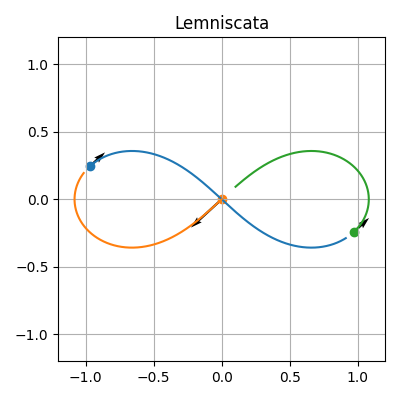
\includegraphics[width=0.35\linewidth]{img/vi/lemniscata.png}
    \end{figure}
\end{probmodelo}

% \begin{probmodelo}[Quatro-folhas com 5 corpos]
%     Problema de 5 corpos com massas unitárias, com um corpo fixado no centro.
%     \begin{figure}[H]
%         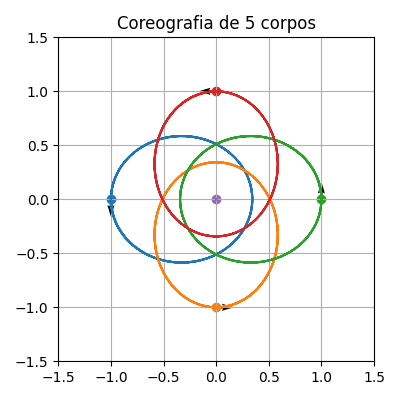
\includegraphics[width=0.35\linewidth]{img/vi/joao_5.png}
%     \end{figure}
% \end{probmodelo}

\begin{probmodelo}[Coreografia-Doicu 5 corpos \cite{Doicu2022}]
    Configuração central de 5 corpos com massas unitárias.
    \begin{figure}[H]
        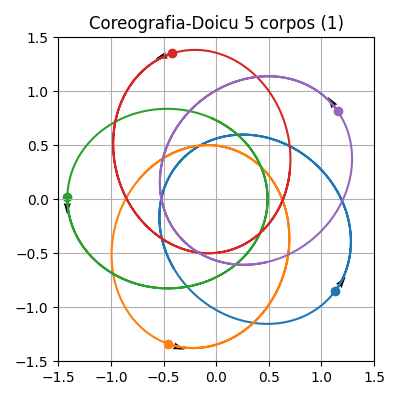
\includegraphics[width=0.35\linewidth]{img/vi/ccnmas5_1.png}
    \end{figure}
\end{probmodelo}

\begin{probmodelo}[Coreografia-Doicu 12 corpos \cite{Doicu2022}]
    Configuração central de 12 corpos com massas $m_a=1/10$, para todo $a = 1, ..., 12$.
    \begin{figure}[h!]
        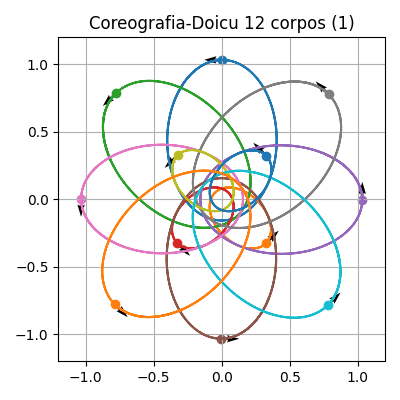
\includegraphics[width=0.35\linewidth]{img/vi/ccnmas12_1.png}
    \end{figure}
\end{probmodelo}

Além disso, para os testes com sorteio de valores iniciais foi utilizada a biblioteca \texttt{ncorpos-vi-py} \cite{ncorpos_vi_py}.

%%%%%%%%%%%%%%%%%%%%%%%%%%%%%%%%%%%%%%%%%%%%%%%%%%%%%%%%%%%%%
\subsection{Resultados esperados}
No PNCG, a parte mais custosa computacionalmente no geral é o cálculo das forças, pois são necessários no mínimo $q = N (N-1) / 2$ cálculos de $\vet F_{a,b}$. Um método de passo único com $R$ estágios faz $Rq$ cálculos, então se estamos aplicando o Parareal com $P$ processadores temos:

Considere
\begin{itemize}
    \item  $k$ iterações;
    \item $\tau_{\mathcal F}$ o tempo computacional para integrar $\delta t$ usando $\mathcal F$;
    \item $\tau_C$ o tempo computacional para integrar $\Delta t$ usando $\mathcal G$; e
    \item $N_p$ o número de processadores em paralelo.
\end{itemize}
Seja também
\begin{equation}\label{eq:parareal_edo_estimativa_ganho}
    S(k) = \dfrac{T_{ref}}{T_{Parareal}(k)}.
\end{equation}
Como visto em aula, $S(k)$ assume o formato:
\begin{equation}
    S(k) = \dfrac{1}{(1+k) \dfrac{\delta t}{\Delta t} \dfrac{\tau_C}{\tau_{\mathcal F}} + \dfrac{k}{N_P}}.
\end{equation}

O principal custo da aplicação de um integrador no problema de N-corpos é o cálculo das $q_N = N(N-1)/2$ forças. Considerando $R_{\mathcal F}$ e $R_C$ o número de estágios dos métodos fino e grosseiro, respectivamente, temos que
\begin{equation}
\dfrac{\tau_C}{\tau_{\mathcal F}} \approx \dfrac{R_C q_N}{R_{\mathcal F} q_N} = \dfrac{R_C}{R_{\mathcal F}}.
\end{equation}
Além disso, consideramos $\delta t = \alpha_t \Delta t$, então
\begin{equation}
    S(k) \approx \dfrac{1}{(1 + k) \alpha_t \dfrac{R_C}{R_{\mathcal F}} + \dfrac{k}{N_P}}.
\end{equation}

...

COISA INTERESSANTE: USAR UM RUNGE-KUTTA 4 COMO FINO E UM RUTH 4 COMO GROSSEIRO MANTÉM ERRO NA MESMA ORDEM, MAS A ENERGIA FICA MELHOR DO QUE O CONTRARIO!

OUTRA COISA INTERESSANTE: USANDO RK4 COMO FINO, O VERLET FICA COM ENERGIA MELHOR QUE O RK2 COMO GROSSEIRO

%%%%%%%%%%%%%%%%%%%%%%%%%%%%%%%%%%%%%%%%%%%%%%%%%%%%%%%%%%%%%
\subsection{Órbitas periódicas}

\subsubsection{Lemniscata}
Para começar, o primeiro valor inicial a ser testado será a lemniscata (p.m. \ref{pm:lemniscata}), um problema de 3 corpos. Testes manuais indicaram que condições razoáveis para testes são usar o intervalo $[0,10]$, tomar $N=200$, $\delta t = 10/(32 N + 1) = 10/6401$ e $\Delta t = 10/(4 N + 1) = 10/801$. Como critério de parada, foi utilizado $\delta t^p$, onde $p$ é a ordem do método fino. Além disso, o MPI foi utilizado com 14 \texit{slots}, sendo um valor razoável encontrado após alguns testes práticos.


\begin{figure}[H]
    \centering
    
    % Linha 1
    \begin{subfigure}{0.45\textwidth}
        \centering
        
\includegraphics[width=\linewidth]{img/t1/rk2_vs_ee/erro_final.png}
        \caption{RK2 vs Euler Explícito}
    \end{subfigure}
    \hfill
    \begin{subfigure}{0.45\textwidth}
        \centering
        
\includegraphics[width=\linewidth]{img/t1/rk2_vs_es/erro_final.png}
        \caption{RK2 vs Euler Simplético}
    \end{subfigure}
    
    \vspace{0.5cm}
    
    % Linha 2
    \begin{subfigure}{0.45\textwidth}
        \centering
        
\includegraphics[width=\linewidth]{img/t1/verlet_vs_ee/erro_final.png}
        \caption{Verlet vs Euler Explícito}
    \end{subfigure}
    \hfill
    \begin{subfigure}{0.45\textwidth}
        \centering
        
\includegraphics[width=\linewidth]{img/t1/verlet_vs_es/erro_final.png}
        \caption{Verlet vs Euler Simplético}
    \end{subfigure}
    
    \vspace{0.5cm}
    
    % Linha 3
    \begin{subfigure}{0.45\textwidth}
        \centering
        
\includegraphics[width=\linewidth]{img/t1/rk4_vs_ee/erro_final.png}
        \caption{RK4 vs Euler Explícito}
    \end{subfigure}
    \hfill
    \begin{subfigure}{0.45\textwidth}
        \centering
        
\includegraphics[width=\linewidth]{img/t1/rk4_vs_es/erro_final.png}
        \caption{RK4 vs Euler Simplético}
    \end{subfigure}
    
    \caption{Erro relativo ao final de cada iteração para os métodos grosseiros de Euler Explícito e Euler Simplético e métodos finos Runge-Kutta 2, Velocity-Verlet e Runge-Kutta 4}
    \label{fig:t1_erro_final}
\end{figure}

Primeiro, conforme a figura \ref{fig:t1_erro_final} é possível ver que o método de Euler Simplético converge mais rapidamente que o método de Euler Explícito mesmo quando não se trata de um método fino simplético. Isso possivelmente decorre de sua maior estabilidade em relação ao método explícito. 

\begin{figure}[H]
    \centering
    
    % Linha 1
    \begin{subfigure}{0.45\textwidth}
        \centering
        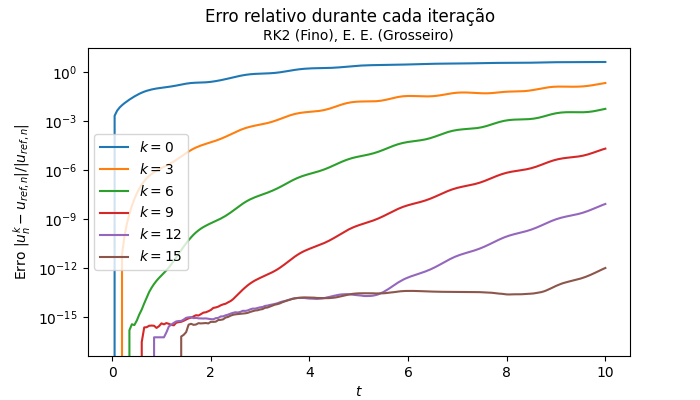
\includegraphics[width=\linewidth]{img/t1/rk2_vs_ee/erro_durante.png}
        \caption{RK2 vs Euler Explícito}
    \end{subfigure}
    \hfill
    \begin{subfigure}{0.45\textwidth}
        \centering
        
\includegraphics[width=\linewidth]{img/t1/rk2_vs_es/erro_durante.png}
        \caption{RK2 vs Euler Simplético}
    \end{subfigure}
    
    \vspace{0.5cm}
    
    % Linha 2
    \begin{subfigure}{0.45\textwidth}
        \centering
        
\includegraphics[width=\linewidth]{img/t1/verlet_vs_ee/erro_durante.png}
        \caption{Verlet vs Euler Explícito}
    \end{subfigure}
    \hfill
    \begin{subfigure}{0.45\textwidth}
        \centering
        
\includegraphics[width=\linewidth]{img/t1/verlet_vs_es/erro_durante.png}
        \caption{Verlet vs Euler Simplético}
    \end{subfigure}
    
    \vspace{0.5cm}
    
    % Linha 3
    \begin{subfigure}{0.45\textwidth}
        \centering
        
\includegraphics[width=\linewidth]{img/t1/rk4_vs_ee/erro_durante.png}
        \caption{RK4 vs Euler Explícito}
    \end{subfigure}
    \hfill
    \begin{subfigure}{0.45\textwidth}
        \centering
        
\includegraphics[width=\linewidth]{img/t1/rk4_vs_es/erro_durante.png}
        \caption{RK4 vs Euler Simplético}
    \end{subfigure}
    
    \caption{Erro relativo durante iterações para os métodos grosseiros de Euler Explícito e Euler Simplético e métodos finos Runge-Kutta 2, Velocity-Verlet e Runge-Kutta 4}
    \label{fig:t1_erro_durante}
\end{figure}

Na figura \ref{fig:t1_erro_durante} é possível ver melhor o impacto da diferença de estabilidade entre os métodos. O método grosseiro simplético apresenta um crescimento de erro menos acentuado com o passar do tempo, enquanto o erro no método explícito cresce mais rapidamente, acumulando mais erros a cada passo das iterações.

\begin{figure}[H]
    \centering
    
    % Linha 1
    \begin{subfigure}{0.45\textwidth}
        \centering
        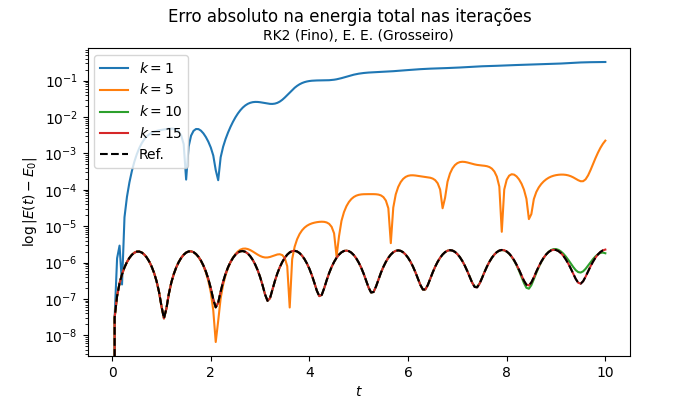
\includegraphics[width=\linewidth]{img/t1/rk2_vs_ee/erro_durante_energia.png}
        \caption{RK2 vs Euler Explícito}
    \end{subfigure}
    \hfill
    \begin{subfigure}{0.45\textwidth}
        \centering
        
\includegraphics[width=\linewidth]{img/t1/rk2_vs_es/erro_durante_energia.png}
        \caption{RK2 vs Euler Simplético}
    \end{subfigure}
    
    \vspace{0.5cm}
    
    % Linha 2
    \begin{subfigure}{0.45\textwidth}
        \centering
        
\includegraphics[width=\linewidth]{img/t1/verlet_vs_ee/erro_durante_energia.png}
        \caption{Verlet vs Euler Explícito}
    \end{subfigure}
    \hfill
    \begin{subfigure}{0.45\textwidth}
        \centering
        
\includegraphics[width=\linewidth]{img/t1/verlet_vs_es/erro_durante_energia.png}
        \caption{Verlet vs Euler Simplético}
    \end{subfigure}
    
    \vspace{0.5cm}
    
    % Linha 3
    \begin{subfigure}{0.45\textwidth}
        \centering
        
\includegraphics[width=\linewidth]{img/t1/rk4_vs_ee/erro_durante_energia.png}
        \caption{RK4 vs Euler Explícito}
    \end{subfigure}
    \hfill
    \begin{subfigure}{0.45\textwidth}
        \centering
        
\includegraphics[width=\linewidth]{img/t1/rk4_vs_es/erro_durante_energia.png}
        \caption{RK4 vs Euler Simplético}
    \end{subfigure}
    
    \caption{Log-erro na energia total durante iterações para os métodos grosseiros de Euler Explícito e Euler Simplético e métodos finos Runge-Kutta 2, Velocity-Verlet e Runge-Kutta 4}
    \label{fig:t1_erro_durante_energia}
\end{figure}

Para a energia total a convergência também é mais rápida. Por não ser simplético, o Parareal apresenta crescimento no erro da energia mesmo quando os método fino e grosseiro são simpléticos. Ainda assim, usar um método grosseiro simplético, ao menos nesse caso, apresentou vantagens sobre o uso de um método grosseiro não simplético.

\begin{figure}[H]
    \centering
    
    % Linha 1
    \begin{subfigure}{0.45\textwidth}
        \centering
        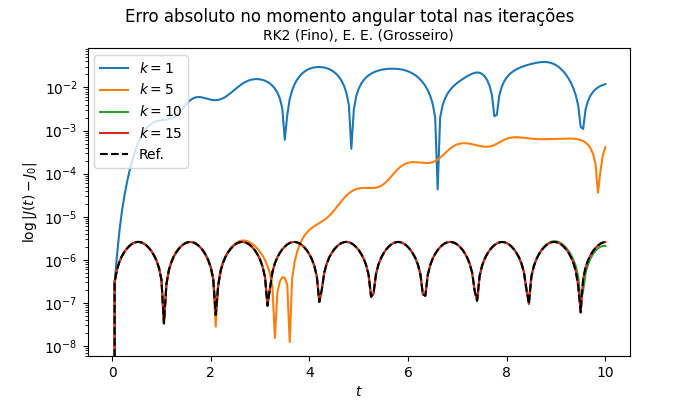
\includegraphics[width=\linewidth]{img/t1/rk2_vs_ee/erro_durante_angular.png}
        \caption{RK2 vs Euler Explícito}
    \end{subfigure}
    \hfill
    \begin{subfigure}{0.45\textwidth}
        \centering
        
\includegraphics[width=\linewidth]{img/t1/rk2_vs_es/erro_durante_angular.png}
        \caption{RK2 vs Euler Simplético}
    \end{subfigure}
    
    \vspace{0.5cm}
    
    % Linha 2
    \begin{subfigure}{0.45\textwidth}
        \centering
        
\includegraphics[width=\linewidth]{img/t1/verlet_vs_ee/erro_durante_angular.png}
        \caption{Verlet vs Euler Explícito}
    \end{subfigure}
    \hfill
    \begin{subfigure}{0.45\textwidth}
        \centering
        
\includegraphics[width=\linewidth]{img/t1/verlet_vs_es/erro_durante_angular.png}
        \caption{Verlet vs Euler Simplético}
    \end{subfigure}
    
    \vspace{0.5cm}
    
    % Linha 3
    \begin{subfigure}{0.45\textwidth}
        \centering
        
\includegraphics[width=\linewidth]{img/t1/rk4_vs_ee/erro_durante_angular.png}
        \caption{RK4 vs Euler Explícito}
    \end{subfigure}
    \hfill
    \begin{subfigure}{0.45\textwidth}
        \centering
        
\includegraphics[width=\linewidth]{img/t1/rk4_vs_es/erro_durante_angular.png}
        \caption{RK4 vs Euler Simplético}
    \end{subfigure}
    
    \caption{Log-erro no momento angular total durante iterações para os métodos grosseiros de Euler Explícito e Euler Simplético e métodos finos Runge-Kutta 2, Velocity-Verlet e Runge-Kutta 4}
    \label{fig:t1_erro_durante_angular}
\end{figure}

Apesar de também ser mais rápida que para o método explícito, a convergência do momento angular total com o método de Euler Simplético precisou de mais passos que para a energia total para os métodos finos Verlet e RK4, que apresentam um erro menor no momento angular do que o método RK2 (o primeiro por ser simplético, e o segundo por ter ordem maior).

Ainda assim, em nenhum caso utilizar o método Parareal foi mais vantajoso que utilizar o método sequencial. Conforme a figura \ref{fig:t1_tempo}, o método Parareal levou entre 4 e 5 vezes mais tempo que a aplicação sequencial do método fino.

\begin{figure}[H]
    \centering
    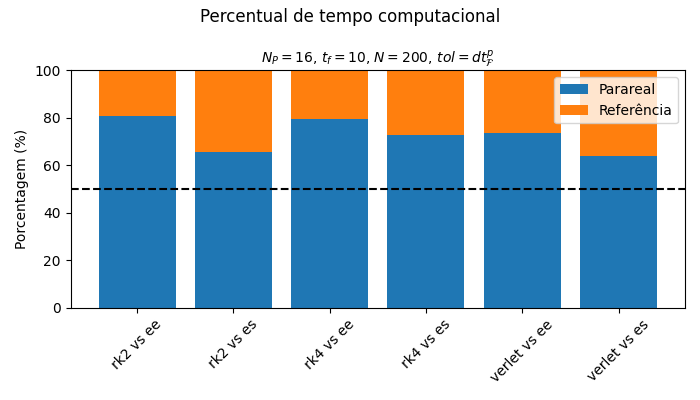
\includegraphics[width=0.6\linewidth]{img/t1/tempo_computacional.png}
    \caption{Percentual de tempo computacional dos métodos aplicados com Parareal e sequencialmente.}
    \label{fig:t1_tempo}
\end{figure}

%%%%%%%%%%%%%%%%%%%%%%%%%%%%%%%%%%%%%%%%%%%%%%%%%%%%%%%%%%%%%%%%%%%%%%%%%%%%%%%%%
\subsubsection{Problema com 5 corpos}

O problema de 5 corpos já não converge tão rapidamente quanto à lemniscata. Por isso, também serão utilizados métodos de segunda ordem como métodos grosseiros.

\begin{figure}[H]
    \centering
    
    % Linha 1
    \begin{subfigure}{0.45\textwidth}
        \centering
        
\includegraphics[width=\linewidth]{img/t2/erro_final.png}
        \caption{Erro final.}
        \label{fig:t2_erros_erro_relativo}
    \end{subfigure}
    \hfill
    \begin{subfigure}{0.45\textwidth}
        \centering
        
\includegraphics[width=\linewidth]{img/t2/erro_final_energia.png}
        \caption{Erro em $E$.}
        \label{fig:t2_erros_erro_energia}
    \end{subfigure}
    
    \vspace{0.5cm}

    \begin{subfigure}{0.45\textwidth}
        \centering
        
\includegraphics[width=\linewidth]{img/t2/erro_final_angular.png}
        \caption{Erro em $J$}
        \label{fig:t2_erros_erro_angular}
    \end{subfigure}
    
    \caption{Log-erros ao final de cada iteração com os métodos finos Runge-Kutta 4 e Ruth4 e métodos grosseiros Euler Simplético, Runge-Kutta 2 e Verlet.}
    
    \label{fig:t2_erros}
\end{figure}

Conforme a figura \ref{fig:t2_erros_erro_relativo}, podemos observar um erro relativo ao final de cada iteração bastante parecido entre os métodos Ruth4 e RK4. Ambos os métodos são de ordem 4, e apesar da diferença geométrica, seus erros relativos curiosamente se comportam de maneira bastante semelhante.

Ainda assim, podemos observar que utilizar um método grosseiro simplético de ordem 2 apresentou um resultado melhor que um grosseiro não simplético. É preciso levar em conta que o método RK2, como o método de Euler Explícito, é instável.

Já o erro na energia, conforme a figura \ref{fig:t2_erros_erro_energia}, é menor para o método fino simplético, como esperado.

O erro no momento angular, conforme a figura \ref{fig:t2_erros_erro_angular}, tem também o resultado esperado. Na iteração zero, quando somente o método grosseiro é aplicado, os métodos simpléticos têm erro de ponto flutuante e o RK2 tem um erro de $10^{-4}$. Da mesma forma, durante as iterações, os métodos simpléticos (grosseiros e fino) apresentam resultado relativamente melhor que o RK2 como grosseiro e o RK4 como fino.

\begin{figure}[H]
    \centering
    
\includegraphics[width=0.6\linewidth]{img/t2/tempo_computacional.png}
    \caption{Percentual de tempo computacional dos métodos aplicados com Parareal e sequencialmente.}
    \label{fig:t2_tempo}
\end{figure}

Sobre a diferença de tempo entre o Parareal e a aplicação sequencial, observamos uma diferença em comparação com o teste 1. Utilizando o método de Verlet como grosseiro, dessa vez, compensou em ambos os casos, embora pouco. Vale ressaltar que por ser um intervalo relativamente pequeno, com relativamente poucas iterações, seria necessária uma amostragem e o gráfico representaria tal amostragem, em vez de uma rodada isolada.

%%%%%%%%%%%%%%%%%%%%%%%%%%%%%%%%%%%%%%%%%%%%%%%%%%%%%%%%%%%%%%%%%%%%%%%%%%%%%%%%%
\subsubsection{Problema com 12 corpos}

Este problema tem um período de aproximadamente $3.5$ unidades de tempo. Com a subdivisão de intervalos anterior, os métodos de quarta ordem não são capazes de sustentar as trajetórias por mais do que 2 períodos. Apesar de o Parareal convergir para as trajetórias do método fino - ainda que estejam erradas -, nesse caso os corpos se entrelaçam e espiralam rapidamente. Nos subintervalos definidos, esse comportamento espiral é oscilatório, então a não convergência do Parareal é esperada.

\begin{figure}[H]
    \centering
    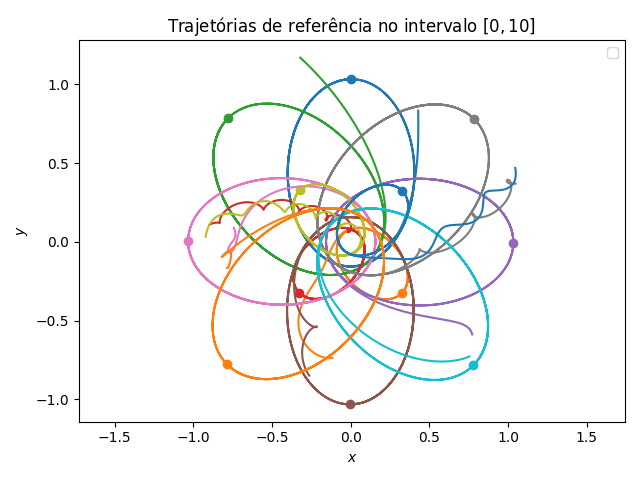
\includegraphics[width=0.6\linewidth]{img/t4/trajetorias_10.png}
    \caption{Trajetórias no intervalo $[0,10]$ via Ruth4 com $\delta t=10/6401$.}
    \label{fig:t4_trajetorias_10}
\end{figure}

Porém, tomando o intervalo $[0,8]$ e os passos $\delta t = 8/6401$ e $\Delta t = 8/201$ (ou seja, com multiplicador do grosseiro sendo 1), os métodos de ordem 4 ficam estáveis e permitem a aplicação do Parareal. Além disso, o resultado curiosamente atinge a ordem de $10^{-11}$ e oscila um pouco antes de conseguir atingir o erro $\delta t^4$; assim, foi escolhido $\delta t^{3.2}$ como um critério de parada, o que continua razoável considerando a quantidade de períodos integrada.

\begin{figure}[H]
    \centering
    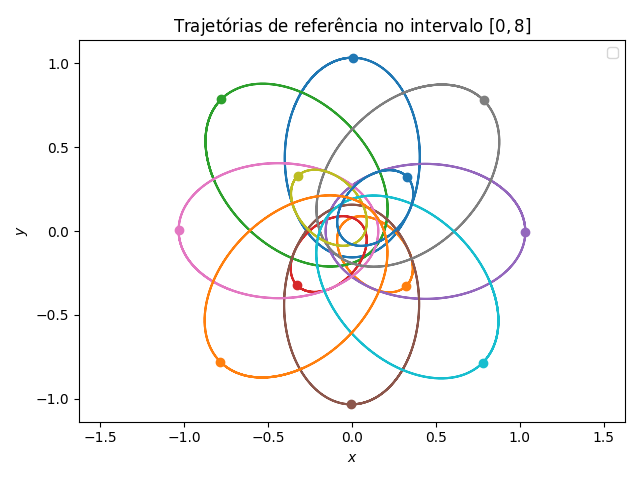
\includegraphics[width=0.6\linewidth]{img/t4/trajetorias_8.png}
    \caption{Trajetórias no intervalo $[0,8]$ via Ruth4 com $\delta t=8/6401$.}
    \label{fig:t4_trajetorias_8}
\end{figure}

Dessa vez, em termos de erros, conforme a figura \ref{fig:t4_erros_erro_relativo}, todos os métodos apresentam um comportamento semelhante em termos de convergência. Já em termos de energia, conforme a figura \ref{fig:t4_erros_erro_energia}, utilizar um método grosseiro simplético oferece alguma diferença, embora não seja tão expressiva a menos da última iteração.

\begin{figure}[H]
    \centering
    
    % Linha 1
    \begin{subfigure}{0.45\textwidth}
        \centering
        
\includegraphics[width=\linewidth]{img/t4/erro_final.png}
        \caption{Erro final.}
        \label{fig:t4_erros_erro_relativo}
    \end{subfigure}
    \hfill
    \begin{subfigure}{0.45\textwidth}
        \centering
        
\includegraphics[width=\linewidth]{img/t4/erro_final_energia.png}
        \caption{Erro em $E$.}
        \label{fig:t4_erros_erro_energia}
    \end{subfigure}
    
    \vspace{0.5cm}

    \begin{subfigure}{0.45\textwidth}
        \centering
        
\includegraphics[width=\linewidth]{img/t4/erro_final_angular.png}
        \caption{Erro em $J$}
        \label{fig:t4_erros_erro_angular}
    \end{subfigure}
    
    \caption{Log-erros ao final de cada iteração com os métodos finos Runge-Kutta 4 e Ruth4 e métodos grosseiros Euler Simplético, Runge-Kutta 2 e Verlet.}
    
    \label{fig:t4_erros}
\end{figure}

O momento angular, por outro lado, apresenta o comportamento esperado, novamente. A diminuição até erro de máquina ocorre somente quando utilizado um método fino simplético, curiosamente ocorrendo mesmo com o método grosseiro RK2.

\begin{figure}[H]
    \centering
    
\includegraphics[width=0.6\linewidth]{img/t4/tempo_computacional.png}
    \caption{Percentual de tempo computacional dos métodos aplicados com Parareal e sequencialmente.}
    \label{fig:t4_tempo}
\end{figure}

Em termos de tempo, dessa vez houve um equilíbrio maior. No entanto, ainda sem ter um ganho realmente significativo.

% [FAZER TESTES COM OS PROBLEMAS PERIÓDICOS, COMEÇANDO PELA LEMNISCATA E PELO QUATRO FOLHAS. ANALISAR CONVERGENCIA, TEMPO E COMPORTAMENTO DAS INTEGRAIS PRIMEIRAS. ANALISAR COMO A VARIAÇÃO DOS PARÂMETROS AFETA O RESULTADO. ÓRBITAS PERIÓDICAS TÊM AUTOVALOR IMAGINÁRIO (PORQUE SÃO OSCILATÓRIAS), ENTÃO PEGAR TRECHOS MENORES PODE SER MAIS INTERESSANTE.]

% [A ESTABILIDADE VAI DEPENDER DOS MÉTODOS UTILIZADOS. NESSE CASO, POSSO COMPARAR O MÉTODO FINO PURO, O MÉTODO GROSSEIRO PURO E O PARAREAL, PARA VER SE O PARAREAL OFERECE VANTAGENS SOBRE O GROSSEIRO PELO MENOS.]

%%%%%%%%%%%%%%%%%%%%%%%%%%%%%%%%%%%%%%%%%%%%%%%%%%%%%%%%%%%%%
%%%%%%%%%%%%%%%%%%%%%%%%%%%%%%%%%%%%%%%%%%%%%%%%%%%%%%%%%%%%%
%%%%%%%%%%%%%%%%%%%%%%%%%%%%%%%%%%%%%%%%%%%%%%%%%%%%%%%%%%%%%
%%%%%%%%%%%%%%%%%%%%%%%%%%%%%%%%%%%%%%%%%%%%%%%%%%%%%%%%%%%%%
%%%%%%%%%%%%%%%%%%%%%%%%%%%%%%%%%%%%%%%%%%%%%%%%%%%%%%%%%%%%%
%%%%%%%%%%%%%%%%%%%%%%%%%%%%%%%%%%%%%%%%%%%%%%%%%%%%%%%%%%%%%
%%%%%%%%%%%%%%%%%%%%%%%%%%%%%%%%%%%%%%%%%%%%%%%%%%%%%%%%%%%%%
\subsection{Órbitas gerais}

% [SORTEAR VALORES INICIAIS COM DIFERENTES PARÂMETROS, OBSERVAR O COMPORTAMENTO GERAL E O TEMPO DE COMPUTAÇÃO. OBSERVAR INTEGRAIS PRIMEIRAS. COMENTAR SOBRE A VALIDADE ESTATÍSTICA DAS SIMULAÇÕES DE N-CORPOS E VERIFICAR SE O PARAREAL MANTÉM ESSA VALIDADE ESTATÍSTICA.]

Ao tratar de órbitas gerais, existem questões sobre a validade das soluções, independente do método escolhido que foram levantadas desde o início das simulações numéricas de N-corpos \cite{Miller1964,Boekholt2015}. No entanto, há validade estatística nas simulações, apesar da divergência para trajetórias individuais \cite{shadoworbits}. Isso sugere que ainda que o método Parareal não convirja para a trajetória esperada, pode ser considerado utilizável caso mantenha a validade estatística da solução.

Para testar isso, vou utilizar a biblioteca \texttt{ncorpos-vi-py} \cite{ncorpos_vi_py} para gerar valores iniciais sob condições de equilíbrio (virial) inicial, isto é,
\begin{equation}
2 T (\vet p_0) + V(\vet q_0) = 0,
\end{equation}
e com integrais primeiras nulas, a menos da energia que será $E=-0.25$. Essas condições são uma padronização escolhida entre os simuladores de N-corpos na década de 1980 para possibilitar a comparação entre as diferentes implementações da época \cites{Heggie}[pp.110-112]{aarseth_gravitational_2003}. Foram gerados valores iniciais sob tais condições para 10, 50 e 200 corpos.

Além disso, como não há garantia de que não haverão colisões ou aproximações intensas, o potencial será amortecido com $\varepsilon = 0.05$. Testes com choques elásticos (junto do amortecimento do potencial) também serão feitos, visando avaliar o comportamento do Parareal sob descontinuidades. 

Os valores iniciais podem ser encontrados em [ADICIONAR REPOSITÓRIO].


%%%%%%%%%%%%%%%%%%%%%%%%%%%%%%%%%%%%%%%%%%%%%%%%%%%%%%%%%%%%%
\subsubsection{Potencial amortecido}

Nesse caso, conforme as figuras \ref{fig:t5_1_erros}, \ref{fig:t5_2_erros} e \ref{fig:t5_3_erros}, o uso do método Parareal não compensou até 50 corpos, exigindo um grande número de iterações para convergir, e inclusive tendo um erro oscilatório ao atingir a casa de $10^{-10}$. Já para o problema de 200 corpos, a convergência foi curiosamente mais veloz, e o custo também passou a ser menor que o custo da aplicação sequencial do método fino, conforme a figura \ref{fig:t5_3_erros}.

O bom comportamento do método Parareal se dá pela estabilidade numérica de um potencial suavizado, com trajetórias sendo curvas suaves e com variações não tão bruscas pelo espaço de fases.

\begin{figure}[H]
    \centering
    
    % Linha 1
    \begin{subfigure}{0.45\textwidth}
        \centering
        
\includegraphics[width=\linewidth]{img/t5_1/erro_final.png}
        \caption{Erro final.}
        \label{fig:t5_1_erros_erro_relativo}
    \end{subfigure}
    \hfill
    \begin{subfigure}{0.45\textwidth}
        \centering
        
\includegraphics[width=\linewidth]{img/t5_1/erro_final_energia.png}
        \caption{Erro em $E$.}
        \label{fig:t5_1_erros_erro_energia}
    \end{subfigure}
    
    \vspace{0.5cm}

    \begin{subfigure}{0.45\textwidth}
        \centering
        
\includegraphics[width=\linewidth]{img/t5_1/erro_final_angular.png}
        \caption{Erro em $J$}
        \label{fig:t5_1_erros_erro_angular}
    \end{subfigure}
    \hfill
    \begin{subfigure}{0.45\textwidth}
        \centering
        
\includegraphics[width=\linewidth]{img/t5_1/tempo_computacional.png}
        \caption{Tempo computacional.}
        \label{fig:t5_1_tempo}
    \end{subfigure}
    
    \caption{Log-erros ao final de cada iteração no problema de 10 corpos.}
    
    \label{fig:t5_1_erros}
\end{figure}

\begin{figure}[H]
    \centering
    
    % Linha 1
    \begin{subfigure}{0.45\textwidth}
        \centering
        
\includegraphics[width=\linewidth]{img/t5_2/erro_final.png}
        \caption{Erro final.}
        \label{fig:t5_2_erros_erro_relativo}
    \end{subfigure}
    \hfill
    \begin{subfigure}{0.45\textwidth}
        \centering
        
\includegraphics[width=\linewidth]{img/t5_2/erro_final_energia.png}
        \caption{Erro em $E$.}
        \label{fig:t5_2_erros_erro_energia}
    \end{subfigure}
    
    \vspace{0.5cm}

    \begin{subfigure}{0.45\textwidth}
        \centering
        
\includegraphics[width=\linewidth]{img/t5_2/erro_final_angular.png}
        \caption{Erro em $J$}
        \label{fig:t5_2_erros_erro_angular}
    \end{subfigure}
    \hfill
    \begin{subfigure}{0.45\textwidth}
        \centering
        
\includegraphics[width=\linewidth]{img/t5_2/tempo_computacional.png}
        \caption{Tempo computacional.}
        \label{fig:t5_2_tempo}
    \end{subfigure}
    
    \caption{Log-erros ao final de cada iteração no problema de 50 corpos.}
    
    \label{fig:t5_2_erros}
\end{figure}

\begin{figure}[H]
    \centering
    
    % Linha 1
    \begin{subfigure}{0.45\textwidth}
        \centering
        
\includegraphics[width=\linewidth]{img/t5_3/erro_final.png}
        \caption{Erro final.}
        \label{fig:t5_3_erros_erro_relativo}
    \end{subfigure}
    \hfill
    \begin{subfigure}{0.45\textwidth}
        \centering
        
\includegraphics[width=\linewidth]{img/t5_3/erro_final_energia.png}
        \caption{Erro em $E$.}
        \label{fig:t5_3_erros_erro_energia}
    \end{subfigure}
    
    \vspace{0.5cm}

    \begin{subfigure}{0.45\textwidth}
        \centering
        
\includegraphics[width=\linewidth]{img/t5_3/erro_final_angular.png}
        \caption{Erro em $J$}
        \label{fig:t5_3_erros_erro_angular}
    \end{subfigure}
    \hfill
    \begin{subfigure}{0.45\textwidth}
        \centering
        
\includegraphics[width=\linewidth]{img/t5_3/tempo_computacional.png}
        \caption{Tempo computacional.}
        \label{fig:t5_3_tempo}
    \end{subfigure}
    
    \caption{Log-erros ao final de cada iteração no problema de 200 corpos.}
    
    \label{fig:t5_3_erros}
\end{figure}


%%%%%%%%%%%%%%%%%%%%%%%%%%%%%%%%%%%%%%%%%%%%%%%%%%%%%%%%%%%%%
\subsubsection{Choques elásticos}

Outra forma de evitar que corpos se aproximem muito é introduzir choques elásticos. Para evitar instabilidades numéricas de aproximações intensas no processo do Parareal, o amortecimento no potencial foi mantido, e os valores iniciais são os mesmos, sob as mesmas condições de equilíbrio inicial.

Para o problema de 10 corpos, conforme a figura \ref{fig:t6_1_erros}, o método convergiu e sem vantagens.

\begin{figure}[H]
    \centering
    
    % Linha 1
    \begin{subfigure}{0.45\textwidth}
        \centering
        
\includegraphics[width=\linewidth]{img/t6_1/erro_final.png}
        \caption{Erro final.}
        \label{fig:t6_1_erros_erro_relativo}
    \end{subfigure}
    \hfill
    \begin{subfigure}{0.45\textwidth}
        \centering
        
\includegraphics[width=\linewidth]{img/t6_1/erro_final_energia.png}
        \caption{Erro em $E$.}
        \label{fig:t6_1_erros_erro_energia}
    \end{subfigure}
    
    \vspace{0.5cm}

    \begin{subfigure}{0.45\textwidth}
        \centering
        
\includegraphics[width=\linewidth]{img/t6_1/erro_final_angular.png}
        \caption{Erro em $J$}
        \label{fig:t6_1_erros_erro_angular}
    \end{subfigure}
    \hfill
    \begin{subfigure}{0.45\textwidth}
        \centering
        
\includegraphics[width=\linewidth]{img/t6_1/tempo_computacional.png}
        \caption{Tempo computacional.}
        \label{fig:t6_1_tempo}
    \end{subfigure}
    
    \caption{Log-erros ao final de cada iteração no problema de 10 corpos.}
    
    \label{fig:t6_1_erros}
\end{figure}

No entanto, com choques elásticos as trajetórias já não são suaves, e o que pode ocorrer é o método grosseiro detectar uma colisão que não é detectada pelo método fino (por erro numérico), fazendo com que o método não convirja (ao menos com um número razoável de passos). Esse foi o caso do problema de 50 corpos quando utilizado um raio $r=0.05$, conforme figura \ref{fig:t6_2_naoconverge_erros_erro_relativo}. 

\begin{figure}[H]
    \centering
    
\includegraphics[width=0.5\linewidth]{img/t6_2_naoconverge/erro_final.png}
    \caption{Erro relativo do problema de 50 corpos com raio 0.05.}
    \label{fig:t6_2_naoconverge_erros_erro_relativo}
\end{figure}

Utilizando um raio $r=0.025$, porém, o método convergiu sem ganhos.

\begin{figure}[H]
    \centering
    
    % Linha 1
    \begin{subfigure}{0.45\textwidth}
        \centering
        
\includegraphics[width=\linewidth]{img/t6_2/erro_final.png}
        \caption{Erro final.}
        \label{fig:t6_2_erros_erro_relativo}
    \end{subfigure}
    \hfill
    \begin{subfigure}{0.45\textwidth}
        \centering
        
\includegraphics[width=\linewidth]{img/t6_2/erro_final_energia.png}
        \caption{Erro em $E$.}
        \label{fig:t6_2_erros_erro_energia}
    \end{subfigure}
    
    \vspace{0.5cm}

    \begin{subfigure}{0.45\textwidth}
        \centering
        
\includegraphics[width=\linewidth]{img/t6_2/erro_final_angular.png}
        \caption{Erro em $J$}
        \label{fig:t6_2_erros_erro_angular}
    \end{subfigure}
    \hfill
    \begin{subfigure}{0.45\textwidth}
        \centering
        
\includegraphics[width=\linewidth]{img/t6_2/tempo_computacional.png}
        \caption{Tempo computacional.}
        \label{fig:t6_2_tempo}
    \end{subfigure}
    
    \caption{Log-erros ao final de cada iteração no problema de 50 corpos.}
    
    \label{fig:t6_2_erros}
\end{figure}

Para o problema de 200 corpos, com um número considerável de choques entre os corpos no início do sistema, mesmo com $r=0.025$ o método não convergiu (figura \ref{fig:t6_3_erros_erro_relativo}).

\begin{figure}[H]
    \centering
    
\includegraphics[width=0.5\linewidth]{img/t6_3/erro_final.png}
    \caption{Erro relativo do problema de 200 corpos com raio 0.05.}
    \label{fig:t6_3_erros_erro_relativo}
\end{figure}
